\section{实验四\ 内存管理与分页}

\subsection{实验目的}

\begin{enumerate}
    \item 了解 Linux 中的页式存储管理,并理解页目录、页表的概念。
    \item 掌握线性地址到物理地址的转换。
    \item 了解 C 语言中的内联汇编。
\end{enumerate}

\subsection{内存地址空间}

逻辑地址(相对地址,虚拟地址):用户程序经过编译、汇编后形成目标代码,目标代码通常采用相对地址的形式,其首地址为0,其余地址都相对于首地址而编址。不能用逻辑地址在内存中读取信息。

物理地址(绝对地址,实地址):内存中存储单元的地址,可直接寻址。

为保证 CPU 执行指令时可正确访问内存单元,需要将用户程序中的逻辑地址转换为运行时可由机器直接寻址的物理地址,这一过程被称为地址重定位。

关于逻辑地址、线性地址与物理地址:Intel 实模式下,逻辑地址就是物理地址;没有启用分页机制时,线性地址就是物理地址。线性地址是逻辑地址到物理地址变换之间的中间层,段中的偏移地址(逻辑地址)加上相应段的基地址构成了线性地址。

\begin{itemize}
    \item 启动分段机制,未启动分页机制:逻辑地址 --> (分段地址转换) --> 线性地址 --> 物理地址
    \item 启动分段和分页机制:逻辑地址 --> (分段地址转换) --> 线性地址 --> (分页地址转换) --> 物理地址
\end{itemize}

\subsection{分页式存储管理}

分页是操作系统中的一种内存管理技术,可使电脑的主存能够使用存储在辅助内存中的数据。操作系统会将辅助内存中的数据分区成固定大小的区块,称为“页”(pages)。当数据不需要在主存中时,操作系统将分页由主存移到辅助内存;当数据被需要时,再将数据取回,加载在主存中。相对于分段,分页允许内存存储于不连续的区块以维持文件系统的整齐。分页是磁盘和内存间传输数据块的最小单位。

\subsection{页表结构}

分页转换功能由内存中的表来描述,该表即是页表 (page table) ,存放在物理地址空间中。页表可看做是简单的 2\^{}20 物理地址数组。线性到物理地址的映射功能可简单地看做是进行数组查找。NEUOS 保护模式下,内存地址长度 32 位。线性地址的高 20 位构成这个数组的索引值,用于选择对应页面的物理(基)地址。线性地址的低 12 位给出了页面中的偏移量,加上页面的基地址最终形成对应的物理地址。

\subsubsection{NEUOS 的两级页表结构}

页表含有 2\^{}20 (1M) 个表项,每项占用 4 字节。如果作为一个表来存放,最多将占用 4MB 的内存,而 NEUOS 仅支持 16MB 内存。为了减少内存占用量,需要使用两级表。高 20 位线性地址到物理地址的转换也被分为两步,每步转换其中 10 个比特。

第一级表称为页目录 (page directory)。页目录本身被存放在 1 页 4K 页面中,具有 2\^{}10 (1K)个 4 字节长度的表项。这些表项指向对应的二级表。线性地址的最高 10 位(位 22~31)用作一级表(页目录)中的索引值来选择 2\^{}10 个二级表之一。

第二级表称为页表 (page table),每个页表的长度也是 1 页,最多含有 1K 个 4 字节的表项。每个 4 字节表项含有相关页面的 20 位物理基地址。二级页表使用线性地址中间 10 位(位 12~21)作为表项索引值,以获取含有页面 20 位物理基地址的表项。该 20 位页面物理基地址和线性地址中的低 12 位(页内偏移)组合在一起就得到分页转换过程的输出值,即对应的最终物理地址。

\begin{figure}[htbp]
    \centering
    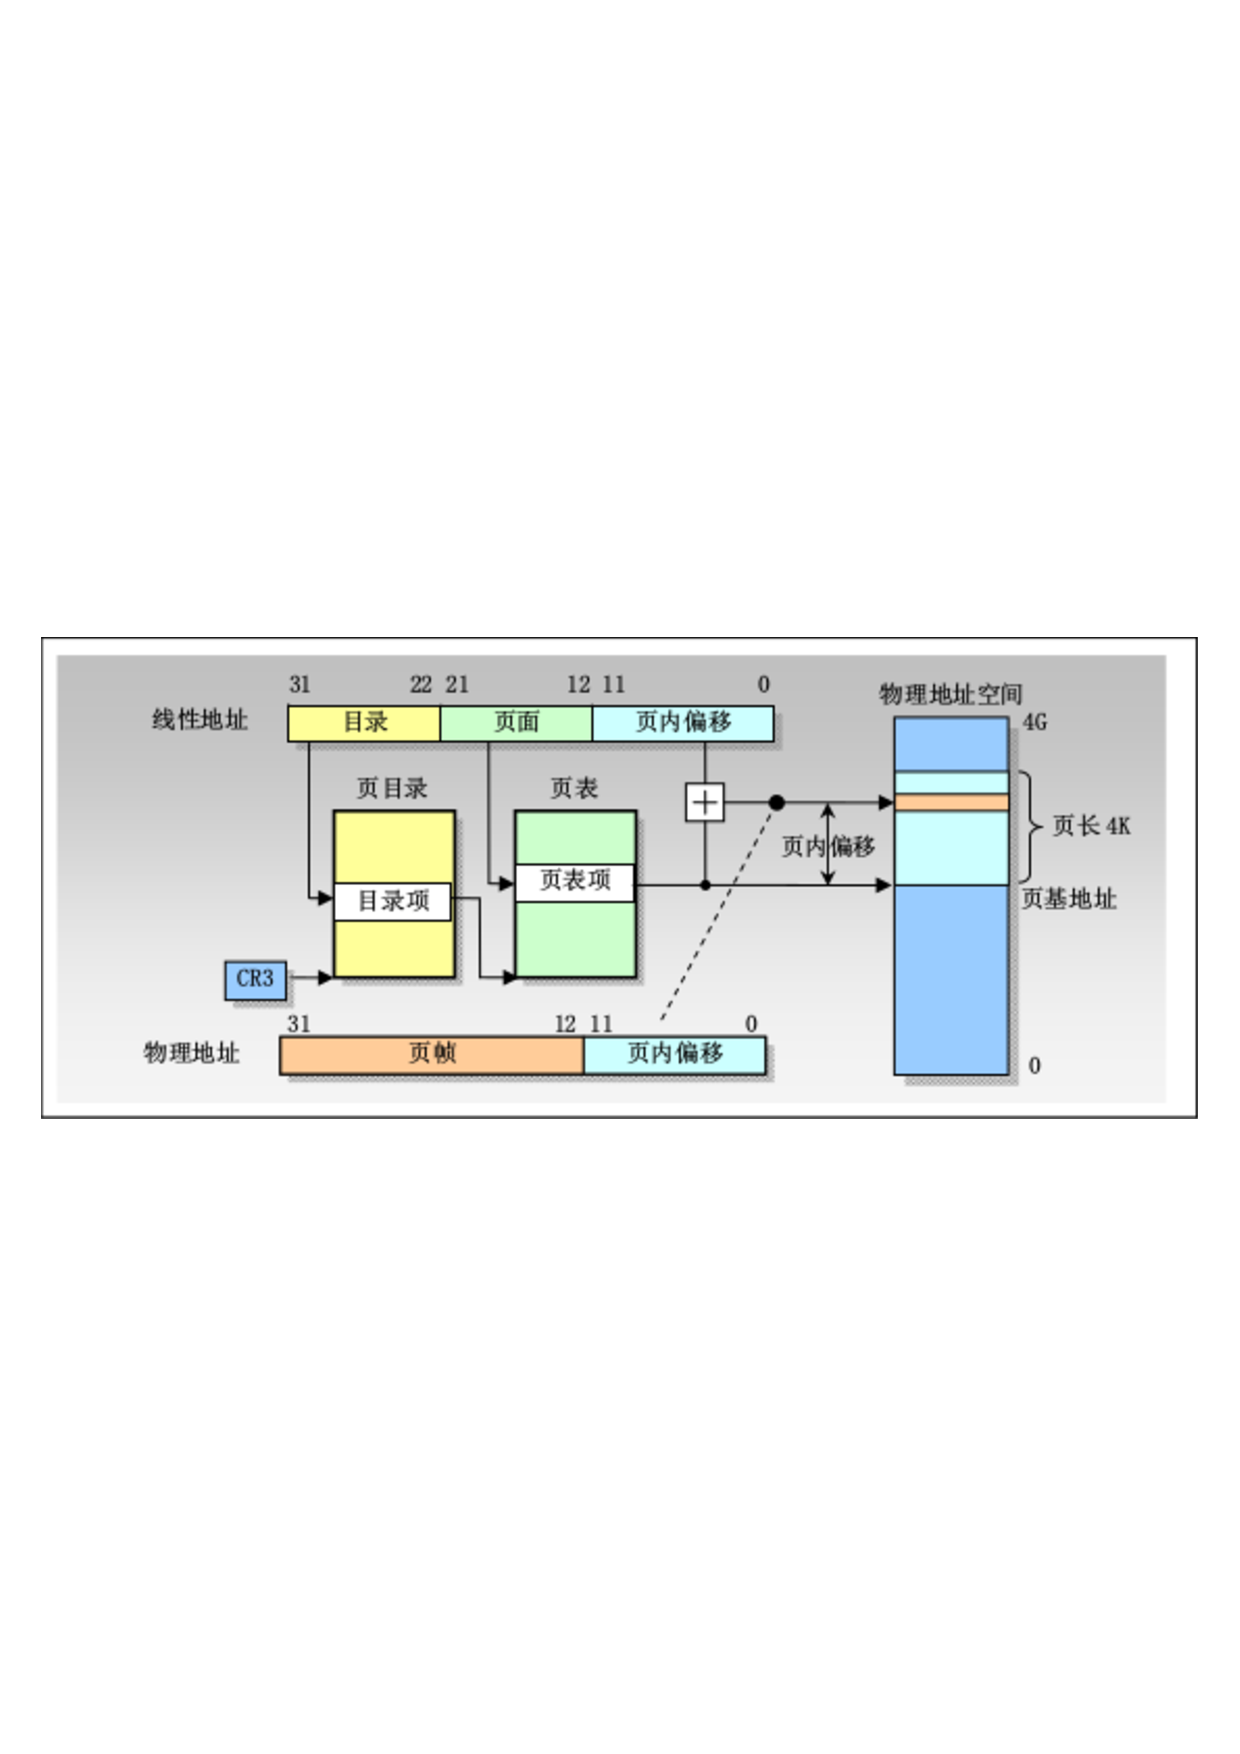
\includegraphics[width=\textwidth]{img/线性地址通过两级页表转换为物理地址.pdf}
    \caption{线性地址通过两级页表转换为物理地址}
    \label{fig:线性地址通过两级页表转换为物理地址}
\end{figure}

二级表结构允许页表被分散在内存各处,而不需要连续保存,而且不需要为不存在的 或线性地址空间未使用部分分配二级页表。

页目录中每个表项都有一个存在 (present) 属性,类似于页表中的表项。页目录表项中的存在属性指明对应的二级页表是否存在。如果存在,直接访问;如果不存在,处理器会产生缺页异常来通知操作系统。页目录表项中的存在属性使操作系统可根据实际使用的线性地址范围来分配二级页表页面。存在位还可用于在虚拟内存中存放二级页表。

\begin{figure}[htbp]
    \centering
    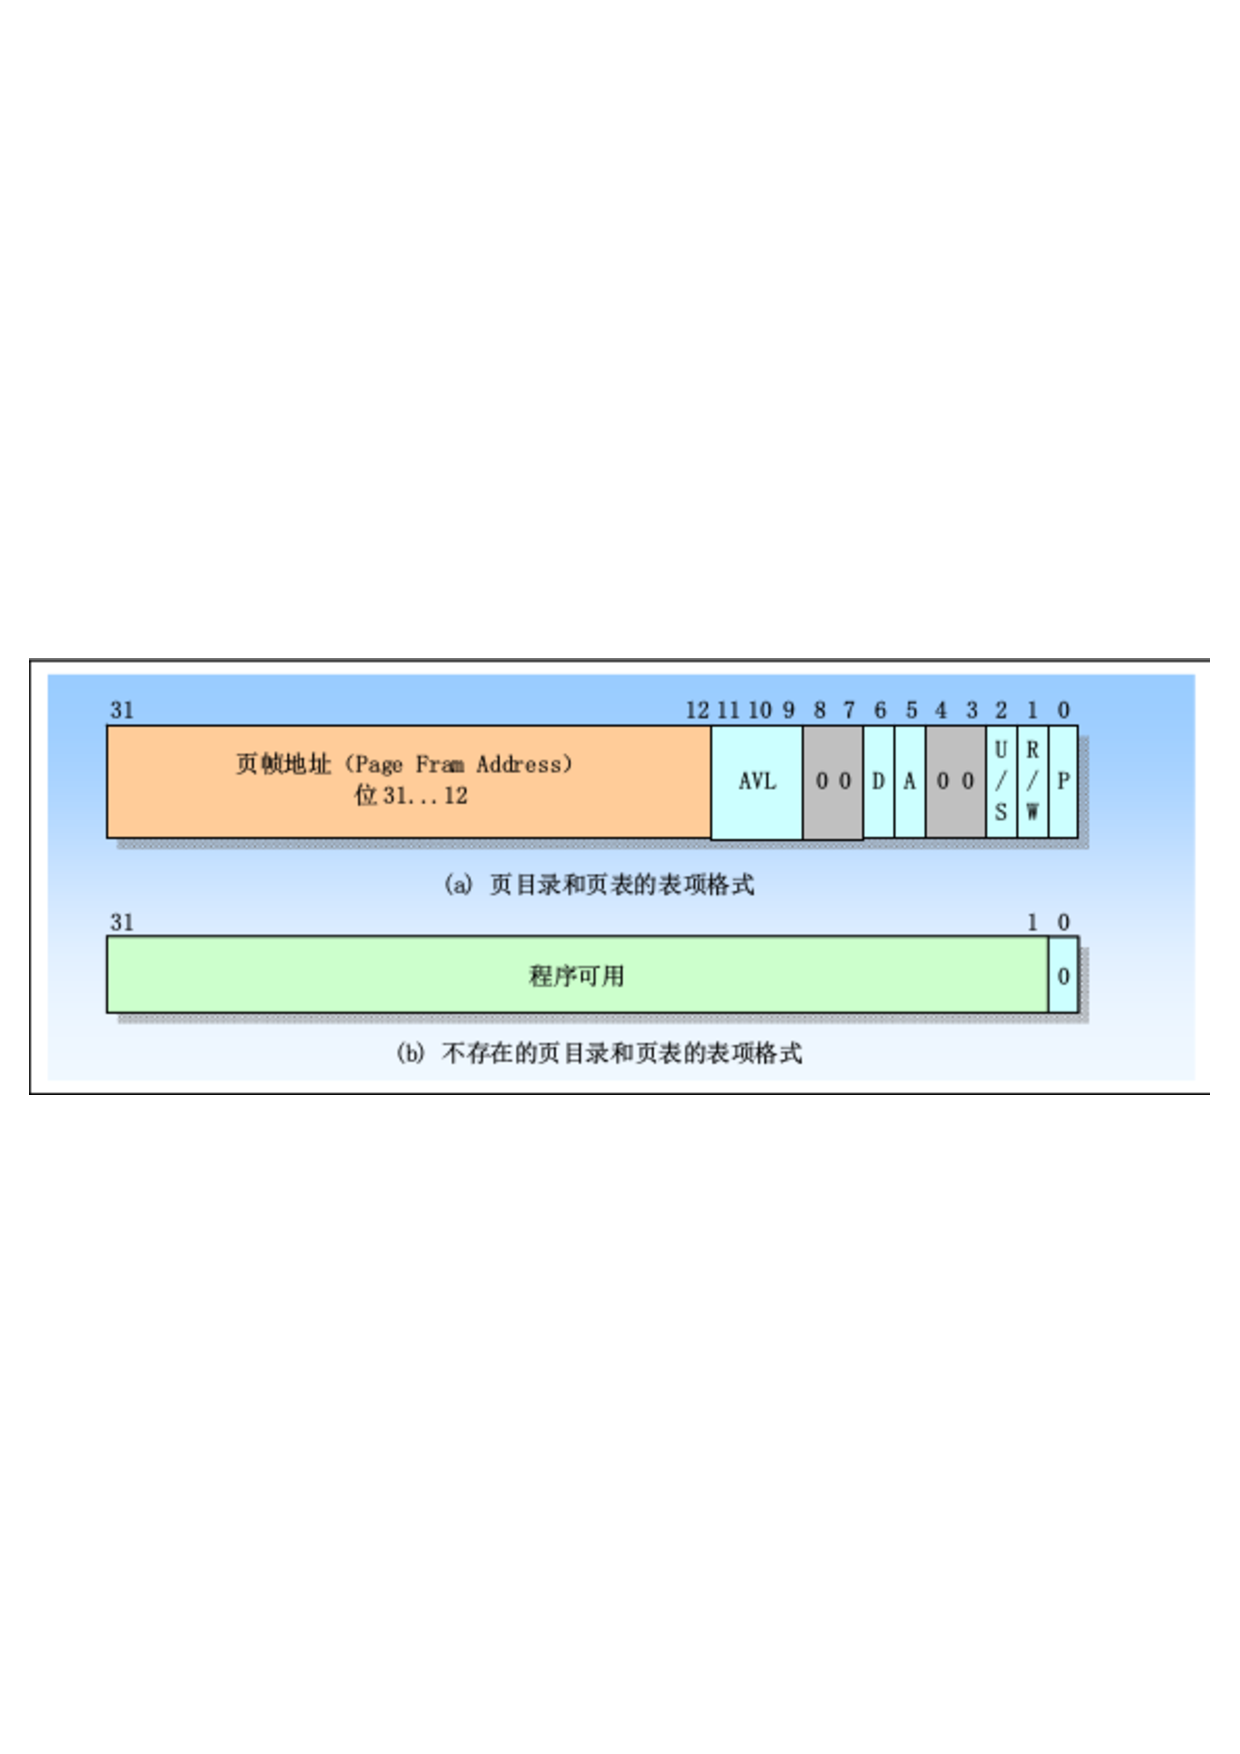
\includegraphics[width=\textwidth]{img/页目录和页表的表项格式.pdf}
    \caption{页目录和页表的表项格式}
    \label{fig:页目录和页表的表项格式址}
\end{figure}

关于表项 0-11 位的意义,见表 \ref{tab:页表项 0-11 位} 的简介。\footnote{\url{https://wiki.osdev.org/Page\_table\#Page\_Table}}

\begin{table}[]
\caption{页表项 0-11 位}
\label{tab:页表项 0-11 位}
\begin{tabular}{llll}
位 & 功能 & 位为 1 & 位为 0 \\
S & 页面大小 & 页面大小是 4M(要求开启 PSE) & 页面大小是 4K \\
A & 访问 & 该页被读或写过 & 该页未被读或写过 \\
D & 缓存禁用 & 该页不会被缓存 & 该页可被缓存 \\
W & 直写/写回 & write through & write back \\
U & 权限 & 用户/Supervisor 均可访问 & 仅 Supervisor 可访问 \\
R & 读写权限 & 可读可写 & 只读 \\
P & 存在 & 该页在物理内存中 & 该页不在物理内存
\end{tabular}
\end{table}

\begin{mdframed}[hidealllines=true,backgroundcolor=gray!20]
\textbf{练习 }PDE(page directory entry) 指页目录项,PTE(page table entry)指页表项。

打开 exp4/mm/mm\_test.c,找到函数 linear\_to\_pte。
该函数的功能是将线性地址通过两级页表转化为物理地址。实现该函数要求使用 C 语言位运算。

请尝试实现该函数,并描述程序通过线性地址获得 pte 的过程。

若转换成功,返回指向页表项的指针;若失败,返回 NULL(0).

在 linear\_to\_pte 函数中,首先使用无符号长整型(32 位)指针 *pde 获取页目录地址;注意,页目录地址不是页目录的索引值,而是内存地址,页目录地址范围是 0x00000000~0x00000fff,每个 PDE 占用内存 4 字节,即查找 PDE 需要将线性地址的前 10 位加上 2 位 0.

然后判断,若 pde 指向的页表不存在(根据 present 位判断) 或者该地址不在页目录地址范围内(页目录地址小于 4 KB),返回 0.

由取内容运算 *pde 取得页目录项存储的地址,由该地址的前 20 位获得页表地址,而后 12 位置为 0,即使得页内偏移为 0;通过线性地址 addr 的 12 - 21 位得到页表索引,页表索引的范围是 0x00000000 ~ 0x003ff000.

最后计算 PTE,由 *pde 取前 20 位得到的页表地址加页表索引,得到指向页表项的指针。页表地址和页表索引的后 12 位均为 0,所得指针存储的地址后 12 位也为 0.
\end{mdframed}

\begin{mdframed}[hidealllines=true,backgroundcolor=gray!20]
\textbf{练习 }打开 exp4/mm/mm\_test.c,找到函数 mm\_print\_pageinfo. 该函数的功能是通过读取页表项显示页的信息。请尝试实现该函数,并描述程序从页表项中获取页的信息的过程。

给定线性地址,尝试读取页表项第 0 位、第 1 位、第 2 位。该函数框架已给出,尝试在该框架内完善;若该页存在于物理内存,\textbf{接着}输出 “P ”,否则不输出;若该页可读可写,\textbf{接着}输出 “R/W ”,否则\textbf{接着}输出 “RO ”;若该页允许 user/supervisor 操作,\textbf{接着}输出 “U/S ”,否则若仅允许 supervisor 操作,\textbf{接着}输出 “U ”。

例如,某页存在于物理内存中,可读可写且允许 user/supervisor 操作,则其 Flag 应输出为 “P R/W U/S”.

\end{mdframed}

\subsection{内联汇编}

内联汇编指的是将汇编语言内嵌在高阶语言的源代码中。这可以提升程序的执行效率,汇编语言代替高阶语言可使代码编写不受编译器的限制;可使程序使用处理器的特有指令;汇编语言能更方便直接地进行系统调用。

GCC提供了两种内联汇编:基本内联汇编语句和扩展内联汇编语句。

\subsubsection{基本内联汇编}

基本内联汇编的基本格式:

\begin{lstlisting}
asm("statements");
# 例如,
asm("nop"); asm("cli");
# “asm”与“__asm__”的含义是完全相同的。
\end{lstlisting}

换行处理:如果有多行汇编,每行末尾要加上“$\backslash n \backslash t$”,即换行符和tab符;目的是使 GCC 将内联汇编代码翻译成一般的汇编代码时能保证换行和留有一定空格。

基本内联汇编的局限:对于基本 asm 语句,双引号内的内容将直接被 GCC 编译成汇编代码,再交给汇编器。如果在内联汇编语句中改变寄存器的值,会影响寄存器原有状态,可能导致程序错误;基本内联汇编也不能实现C语言变量与寄存器内容的交换。

\subsubsection{扩展内联汇编}

一个基本但重要的区别是,简单内联汇编只包括指令,而扩展内联汇编包括操作数。

扩展内联汇编的基本格式:

\begin{lstlisting}
asm [volatile] ( 
Assembler Template
[ : Output Operands ]
[ : Input Operands ]
[ : Clobbers ]
);
# []中表示参数是可选的。
\end{lstlisting}

asm 表示汇编代码的开始,其后所跟的 volatile 是可选项,其含义是避免 asm 指令被删除、移动或组合。在执行代码时,若不希望汇编语句被 GCC 优化而改变位置,就需要添加 volatile 关键字。

volatile 与 \_\_volatile\_\_ 同义。

括号中的语句被“:”分隔为四个部分,第一部分是汇编代码本身,称为指令部,这是必填语句,其他部分均可选。

指令部:在指令部中,加上前缀‘\%’的数字(如\%0,\%1)表示的是需要使用寄存器的\textbf{样板操作数}。在涉及具体寄存器时,寄存器名前应加上两个百分号‘\%\%’,以免产生混淆。

输出部:输出部规定的是输出变量与样板操作数结合的条件,每个条件称为一个\textbf{约束},每个约束以等号起始,可包含多个约束,相互之间用逗号分隔。例如

\begin{lstlisting}
:"=r"(b), "=r"(c)
\end{lstlisting}

其中,b 和 c 是C语言变量,r是限定符,将在下文提到。

输入部:输入约束的格式和输出约束相似,但不带等号。例如,:"r"(b), "r"(c)

声明产生副作用的寄存器:在进行某些操作时,除了进行数据输入和输出的寄存器外,还要使用多个寄存器保存中间的计算结果,这样难免修改原有寄存器的内容。在最后这一部分,对产生副作用的寄存器进行说明,使 GCC 采取相应措施保证寄存器原有状态不受内联汇编语句的影响。例如,:"\%ecx", "\%eax"

操作数编号:在内联汇编中用到的操作数从\textbf{输出部}的第一个约束开始编号,序号从0开始,每个约束记数一次,指令部要引用这些操作数时,只需在序号前加上'\%'作为前缀即可。

限定符:内联汇编语句的指令部在引用一个操作数时总是将其作为32位的长字使用,但实际情况可能需要的是字或字节,因此应该在约束中指明正确的限定符,如表 \ref{tab:限定符} 所示。

\begin{table}[]
\caption{限定符}
\label{tab:限定符}
\begin{tabular}{ll}
限定符 & 含义 \\
"m", "v", "o" & 内存单元 \\
"r" & 任何寄存器 \\
"q" & 寄存器 eax, ebx, ecx, edx 之一 \\
"i", "h" & 直接操作数 \\
"E" 和 "F" & 浮点数 \\
"g" & 任意 \\
"a", "b", "c", "d" & 分别表示寄存器 eax、ebx、ecx 和 edx \\
"S" 和 "D" & 寄存器 esi、edi \\
"I" & 常数(0至31)
\end{tabular}
\end{table}

一段内联汇编的示例:\footnote{Linux 汇编语言开发指南:\url{https://www.ibm.com/developerworks/cn/linux/l-assembly/index.html}}
\footnote{GCC 扩展内联汇编 · ucore\_os\_docs:\url{https://chyyuu.gitbooks.io/ucore\_os\_docs/content/lab0/lab0\_2\_3\_1\_4\_extend\_gcc\_asm.html}}
\footnote{Using the GNU Compiler Collection (GCC): Extended Asm:\url{https://gcc.gnu.org/onlinedocs/gcc/Extended-Asm.html}}

\begin{lstlisting}
/* inline.c */
int main()
{
    int a = 10, b = 0;
    __asm__ __volatile__("movl %1, %%eax;\n\t"
                         "movl %%eax, %0;"
                         :"=r"(b)      /* 输出 */    
                         :"r"(a)       /* 输入 */
                         :"%eax");     /* 不受影响的寄存器 */
     
    printf("Result: %d, %d\n", a, b);
}

// 该程序的功能是将 C 语言变量 a 的值赋给 b.
\end{lstlisting}

\begin{mdframed}[hidealllines=true,backgroundcolor=gray!20]
\textbf{练习 }打开 exp4/mm/mm\_test.c,找到函数 mm\_test\_main. 这个函数用于演示内存管理的各项操作。

参考 4.4 节中对扩展内联汇编的介绍,尝试在这个函数中编写一段内联汇编,修改线性地址 0xdad233 处的内容。

在 mm\_test\_main 函数中,该页被设置为只读且 cr0 寄存器中 WP 位被置位,因此测试这段内联汇编的方法是观察其是否触发了页的写入保护。
\end{mdframed}

\begin{mdframed}[hidealllines=true,backgroundcolor=gray!20]
\textbf{练习 }阅读《Understanding the Linux Virtual Memory Manager》 Chapter 3  Page Table Management\footnote{\url{https://www.kernel.org/doc/gorman/html/understand/understand006.html}},简要论述现代 Linux 与 NEUOS 在页表管理上的不同之处。
\end{mdframed}

\begin{mdframed}[hidealllines=true,backgroundcolor=gray!20]
\textbf{拓展学习 }打开 exp4/mm/memory.c,找到函数 get\_free\_page.

该函数是内联汇编编写的,请尝试将它改写为 C 语言函数,写在 exp4/mm/get\_free\_page.c 源文件中。
\end{mdframed}
